\documentclass{article}
\usepackage[ruled,vlined]{algorithm2e}
\usepackage[bottom=8em]{geometry}
\usepackage{amsmath, amssymb, amsthm, enumerate, hyperref}
\usepackage{color}
\usepackage{setspace}
\usepackage{fancyhdr,lastpage}
\usepackage{url}
\usepackage{tabularx}
\usepackage{tikz}
\pagestyle{fancy}
\lhead{\footnotesize Problem Set 1}
\chead{}
\rhead{\footnotesize CS 4150 - Fall 2020}
\lfoot{}
\cfoot{\small \thepage/\pageref*{LastPage}}
\rfoot{}

\usepackage{graphicx}

\newcommand{\pname}[1]{\textnormal{\textsc{#1}}}

\newtheorem*{theorem}{Theorem}
\newtheorem{definition}{Definition}
\newtheorem*{lemma}{Lemma}


\begin{document}

{\it Please enter your name and uID below.}

\vspace{3em}

\makebox[4.3cm]{Name: Qianlang Chen}
\par
\makebox[4.3cm]{uID: u1172983}
\par

\vfill

\subsubsection*{Submission notes}
\begin{itemize}
  \item Due at 11:59 pm on Friday, September 11.
  \item Solutions must be typeset using one of the template files. For each problem, your answer must fit in the space provided (e.g. not spill onto the next page) *without* space-saving tricks like font/margin/line spacing changes.
  \item Upload a PDF version of your completed problem set to Gradescope.
  \item Teaching staff reserve the right to request original source/tex files during the grading process, so please retain these until an assignment has been returned.
  \item Please remember that for problem sets, collaboration with other students must be limited to a high-level discussion of solution strategies. If you do collaborate with other students in this way, you must identify the students and describe the nature of the collaboration. You are not allowed to create a group solution, and all work that you hand in must be written in your own words. Do not base your solution on any other written solution, regardless of the source.
\end{itemize}

\pagebreak


\begin{enumerate}

  \item (Big-$\Theta$) Proof: to use the definition of Big-$\Theta$, we need to show both $\log(n!) = O[n\log(n)]$ and $\log(n!) = \Omega[n\log(n)]$.

    \begin{itemize}
      \item \textbf{Part I:} show that $\log(n!) = O[n\log(n)]$, that is, there exist constants $c, k > 0$ such that $\log(n!) \le c \cdot n\log(n)$ for all $n \ge k$.

        Proof: let $c = 1$ and $k = 100$. Now, for all $n \ge 100$, we have
        $$
          \begin{aligned}
            \log(n!)      & \le 1 \cdot n\log(n)                                        \\
            \log(n!)      & \le \log(n^n)                                               \\
            10^{\log(n!)} & \le 10^{\log(n^n)}                                          \\
            n!            & \le n^n                                                     \\
            \underbrace{n \cdot (n-1) \cdot (n-2) \cdots 1}_{n\text{ items}}
                          & \le \underbrace{n \cdot n \cdot n\cdots n}_{n\text{ items}}
          \end{aligned}
        $$
        (Since each factor gets smaller on the left-hand side whereas it stays constant on the right-hand side.)

        Therefore, by definition of Big-Oh, $\log(n!) = O[n\log(n)]$.

      \item \textbf{Part II:} show that $\log(n!) = \Omega[n\log(n)]$, that is, there exist constants $c, k > 0$ such that $\log(n!) \ge c \cdot n\log(n)$ for all $n \ge k$.

        Proof: let $c = \frac{1}{4}$ and $k = 100$. Now, for all $n \ge 100$, we have
        $$
          \begin{aligned}
            \log(n!)      & \ge \frac{1}{4} \cdot n\log(n)                                                      \\
            \log(n!)      & \ge \log(n^{\frac{n}{4}})                                                           \\
            10^{\log(n!)} & \ge 10^{\log(n^{n/4})}                                                              \\
            n!            & \ge n^\frac{n}{4}                                                                   \\
            n!            & \ge (\sqrt{n})^{\frac{n}{2}}                                                        \\
            \underbrace{n \cdot (n-1) \cdots (\frac{n}{2}+1)}_{\frac{n}{2}\text{ items}}
            \cdot \frac{n}{2} \cdots 1
                          & \ge \underbrace{\sqrt{n} \cdot \sqrt{n} \cdots \sqrt{n}}_{\frac{n}{2}\text{ items}}
          \end{aligned}
        $$
        (Since $\frac{n}{2} > \sqrt{n}$ for all $n \ge 100$, meaning that the first $\frac{n}{2}$ factors on the left-hand side are all greater than $\sqrt{n}$.)

        Therefore, by definition of Big-$\Omega$, $\log(n!) = \Omega[n\log(n)]$.
    \end{itemize}

    Since we have managed to show both $\log(n!) = O[n\log(n)]$ and $\log(n!) = \Omega[n\log(n)]$, by definition of Big-$\Theta$, $\log(n!) = \Theta[n\log(n)]$. $\square$

    \pagebreak

  \item (Party Planning) \textbf{(a)} Proof: first, this algorithm's result is guaranteed to not contain a single lonely person, because the algorithm would've uninvited that person from the \texttt{while} loop which constantly checks for lonely people.

    Moreover, this algorithm's result is guaranteed to be the \textit{largest} correct subset. The algorithm starts with the complete set of friends and uninvites a person only if it's necessary, that is, only if that person does not have enough friends. It then stops at the first moment when everyone in the invite-list has enough friends, meaning that the subset cannot possibly have a single extra person that is not lonely because the algorithm would've stopped by then.

    Combining the above two points, the algorithm is correct as it always returns the largest subset of friends in which no one is lonely. $\square$

    \textbf{(b)} The basic idea is to use a Depth-First Search. Using Java's terminologies, let us set up the local variables and helper functions as follows:
    \begin{itemize}
      \item \texttt{invited} is a \texttt{LinkedHashMap<String, Vertex>}, representing a graph of friendships with each person being a vertex and each friendship being an edge.
        \begin{itemize}
          \item The \texttt{Vertex} class has the following fields:\\
            \texttt{bool visited, int indegree, ArrayList<Vertex> adjVertices}.
          \item We assume that the input of the program gives a list of names, and the \texttt{String} here keeps track of them.
          \item A \texttt{LinkedHashMap} allows $O(1)$-time insertion and lookup, and it's more friendly for traversal than a regular hash-map.
        \end{itemize}
      \item \texttt{initialize()} takes in a list of edges as the friendships. It sets up the \texttt{invited} graph so that each vertex has the friends of that person being in the \texttt{adjVertices} and the number of friends being the \texttt{indegree}. (Time complexity: $O(n)$ with $n$ being the number of edges/friendships.)
      \item Before the \texttt{while} loop, setup a \texttt{Stack<Vertex>} for the Depth-First Search. It initially contains vertices with \texttt{indegree} of four or less. (Time complexity for adding initial values: $O(n)$ since the number of vertices is at most $2n$ for this problem.)
      \item Perform the DFS: \texttt{while} the stack is not empty (meaning there are still lonely people to uninvite), pop the stack and call \texttt{uninvite()} on the element.
        \begin{itemize}
          \item \texttt{uninvite()} takes in a \texttt{Vertex}, marks it as \texttt{visited}, goes through its \texttt{adjVertices}, and for each \textit{unvisited} adjacent vertex, decrements its \texttt{indegree}, and adds it to the stack if its \texttt{indegree} becomes four or less.
          \item The time complexity of a DFS is $O(n)$ (or more precisely, $O(|V| + n)$, but the number of vertices is at most $2n$ for this problem).
        \end{itemize}
      \item Finally, \texttt{convert\_to\_set()} returns a set of the friend names whose representative vertices are not \texttt{visited} (a vertex is only marked \texttt{visited} when it's detected lonely). (Time complexity: $O(n)$.)
    \end{itemize}

    Since all the sub-procedures described above run in at most $O(n)$, the total run time of the algorithm is $O(n)$ with this setup. $\square$

    \pagebreak

  \item (Amortized ArrayList) Proof: the \texttt{ArrayList} needs to resize once the number of contained elements reaches $n$; so does it once it reaches $(n + c), (n + 2c)$, and so on. During $k$ \texttt{add\_end()} calls, the \texttt{ArrayList} has to resize approximately $\frac{k-n}{c}$ times, since each resize gives it the space for $c$ additional elements. (The error in the number of times it needs to resize due to $(k - n)$ not being a multiple of $c$ will get smaller as $k$ gets large.) Since the \texttt{ArrayList} needs to resize so many times when $k$ is large, the run time of $k$ \texttt{add\_end()} function calls is dominated by the time spent resizing and copying the elements:
    $$
      \begin{aligned}
        T(k) & \approx \overbrace{n + (n + c) + (n + 2c) + \cdots}^{\sim (k-n) / c\text{ items}} \\
             & \approx (\frac{k-n}{c}) \cdot n + (c + 2c + \cdots + (\frac{k-n}{c} - 1) \cdot c) \\
             & \approx \frac{kn-n^2}{c} + c \cdot (1 + 2 + \cdots + (\frac{k-n}{c} - 1))         \\
             & \approx \frac{kn-n^2}{c} + c \cdot \frac{1}{2}(\frac{k-n}{c} - 1)(\frac{k-n}{c})  \\
             & \approx \frac{kn-n^2}{c} + \frac{c}{2}((\frac{k-n}{c})^2 - \frac{k-n}{c})         \\
             & \approx \frac{kn-n^2}{c} + \frac{k^2 - 2kn + n^2}{2c} - \frac{k-n}{c}             \\
             & \approx \boxed{\frac{k^2 - n^2 - 2k - 2n}{2c}}
      \end{aligned}
    $$

    Since $T(k) \ge \frac{1}{4c} \cdot k^2$ for all $k \ge 2n^2 + 4n + 4$, by definition of Big-$\Omega$, $T(k) = \Omega(k^2)$. Therefore, $T(k)$ is not $O(k)$. $\square$

    \pagebreak

  \item (Sorting) Proof: the first thing to observe is that the run time of the \texttt{sorted()} function is $O(r)$ in the worst case, where $r$ is the value of the \texttt{right} input.

    Now, let's consider the worse-case scenario for the entire algorithm.

    \texttt{mergesort2()} is mostly the same as a regular merge-sort, and the only difference is that this new algorithm calls the \texttt{sorted()} function at each recursion level before the regular routine. In the worse-case, the \texttt{sorted()} function returns \texttt{false} every time, forcing the algorithm to do the regular merge-sort. Following this idea, let $T(n, l, r)$ represent the run time of \texttt{mergesort2()} with data size $n$ and values of the arguments \texttt{left} and \texttt{right} being $l$ and $r$, and we have
    $$
      \begin{aligned}
        T(n, l, r) & = T_{\text{sorted}}(r) + T(\frac{n}{2}, l, \frac{l+r}{2})
        + T(\frac{n}{2}, \frac{l+r}{2}, r) + T_{\text{merge}}(n)                                          \\
                   & = O(r) + T(\frac{n}{2}, l, \frac{l+r}{2}) + T(\frac{n}{2}, \frac{l+r}{2}, r) + O(n); \\
        T(n)       & = T(n, 0, n)
      \end{aligned}
    $$
    This is better visualized with the following recursion tree, where the values in each node is formatted as $\boxed{T_{\text{sorted}}(r) + T_{\text{merge}}(n)}$:

    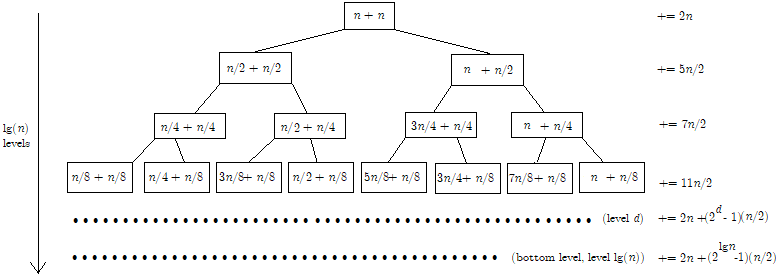
\includegraphics[width=\linewidth]{./images/q4_1.png}

    The total run time of \texttt{mergesort2()} is the sum of the run times for all levels, the values to the right of the tree:
    $$
      \begin{aligned}
        T(n) & = \overbrace{2n + \frac{5n}{2} + \frac{7n}{2} + \frac{11n}{2} + \cdots}^{\log_2(n)\text{ items}}      \\
             & = 2n + (2n + \frac{n}{2}) + (2n + \frac{3n}{2}) + (2n + \frac{7n}{2})
        + \cdots + (2n + (2^{\log_2(n)}-1)\frac{n}{2})                                                               \\
             & = \log_2(n) \cdot 2n + (\frac{n}{2} + \frac{3n}{2} + \frac{7n}{2}
        + \cdots + (n - 1)\frac{n}{2})                                                                               \\
             & = 2n\log_2(n) + (\frac{2n}{2} - \frac{n}{2} + \frac{4n}{2} - \frac{n}{2} + \frac{8n}{2} - \frac{n}{2}
        + \cdots+ n\frac{n}{2} - \frac{n}{2})                                                                        \\
             & = 2n\log_2(n) + \frac{n}{2} \cdot (2 + 4 + 8 + \cdots + n) - \frac{n}{2} \cdot \log_2(n)              \\
             & = \frac{3n\log_2(n)}{2} + n(n - 1) = \boxed{\frac{3n\log_2(n)}{2} + n^2 - n}
      \end{aligned}
    $$

    Now, since we have $T(n) \le 2n^2$ for all $n \ge 1$, by definition of Big-Oh, $T(n) = O(n^2)$. $\square$

    \pagebreak

  \item (Erickson 1.37) \textbf{(a)} As follows:
    \begin{center}
      \begin{minipage}{0.875\linewidth}
        \begin{algorithm}[H]
          \caption{\tt largest\_complete\_subtree}
          \KwIn{\tt BinaryNode curr}
          \KwOut{\tt (BinaryNode root, int depth)}

          \texttt{\\}

          \If{\texttt{curr} is null}
          {
            \Return{\tt (null, -1)}
          }

          \texttt{\\}

          $\texttt{left\_result} \gets \texttt{largest\_complete\_subtree(curr.left)}$

          $\texttt{right\_result} \gets \texttt{largest\_complete\_subtree(curr.right)}$

          \texttt{\\}

          \If{the two resulting depths are equal}
          {
            \If{the two resulting roots are \texttt{curr}'s two children}
            {
              \Return{\tt (curr, left\_result.depth + 1)}
            }
            \Else
            {
              \Return{\tt left\_result}
            }
          }

          \texttt{\\}

          \If{\texttt{left\_result.depth} is greater than \texttt{right\_result.depth}}
          {
            \Return{\tt left\_result}
          }
          \Else
          {
            \Return{\tt right\_result}
          }
        \end{algorithm}
      \end{minipage}
    \end{center}

    \textbf{(b)} Proof: Let's define that, when the input is \texttt{null}, its largest complete subtree (LCS) has a \texttt{null} root and a depth of -1. This doesn't make much sense, but based on the algorithm, this implies that the LCS for a node with no children is rooted at itself with a depth of 0, which is correct for a base case.

    Imagine a node $N$ with at least one child. For an inductive hypothesis, let's assume that the algorithm always returns correct results when called with either of its children $L$ and $R$. Now, there are several possible scenarios:
    \begin{itemize}
      \item If the LCS for both children have the same depth $d$ and are rooted at $L$ and $R$, then $N$ is complete. Thus, the LCS for $N$ is rooted at $N$ with depth $(d + 1)$, which is correct for the algorithm.
      \item If the LCS for both children have the same depth but are not both rooted at the children, then $N$ is incomplete. Thus, both of the resulting LCS are valid answers for the LCS for $N$, which is correct for the algorithm.
      \item If the LCS for both children don't have the same depth, then $N$ is incomplete. The answer here should be whichever resulting LCS with the largest depth, which is correct for the algorithm.
    \end{itemize}
    Therefore, the algorithm always returns the correct results when called with $N$, completing the inductive step. $\square$

    \textbf{(c)} The worst-case input for this algorithm is a tree with all nodes only having a left-child, except for the one leaf. If the input size was $n$, the algorithm would be forced to call itself $n$ times for the left children alone, each time with an input-size-decrease of only one:
    $$T(n) = T(n - 1) + O(1)$$
    Which simplifies to $T(n) = O(n)$ (algebra work omitted). $\square$

\end{enumerate}

\end{document}
